\documentclass[12pt,reqno]{amsart}
%%%%%%%%%%%%%%%%%%%%%%%%%%%%%%%%%%%%%%%%%%%%%%%%%%%
%								Packages									         %
%%%%%%%%%%%%%%%%%%%%%%%%%%%%%%%%%%%%%%%%%%%%%%%%%%%
\usepackage[T1]{fontenc}
\usepackage{amsmath, amssymb, amsthm, amscd, amsfonts}
\usepackage{mathtools}
\usepackage{enumerate,multicol}
\usepackage[shortlabels]{enumitem}

\usepackage[dvipsnames]{xcolor}
\definecolor{DartmouthGreen}{HTML}{00693E}
\definecolor{DartmouthDarkGreen}{HTML}{004B23}
\definecolor{DartmouthLightGreen}{HTML}{4BAF7A}

\usepackage[
  colorlinks=true,
  hyperindex,
  linkcolor=DartmouthDarkGreen,
  citecolor=DartmouthGreen,
  urlcolor=DartmouthGreen,
  pagebackref=true
]{hyperref}

\usepackage{parskip}
\usepackage[letterpaper, margin=.5in, top=1in, bottom=1.4in, headheight=42pt, headsep=14pt, footskip=50pt]{geometry}
\linespread{1.1}

\usepackage{algorithm,algpseudocode,verbatim}
\usepackage{float,caption,comment}

\usepackage{tikz,tikz-cd}
\usetikzlibrary{graphs, graphs.standard,positioning}



\usepackage{calrsfs}
\DeclareMathAlphabet{\pazocal}{OMS}{zplm}{m}{n}
\usepackage{newcent,fouriernc}

%%%%%%%%%%%%%%%%%%%%%%%%%%%%%%%%%%%%%%%%%%%%%%%%%%%
%								Copyright 								         %
%%%%%%%%%%%%%%%%%%%%%%%%%%%%%%%%%%%%%%%%%%%%%%%%%%%
\usepackage{ccicons}
\usepackage{fancyhdr}

\pagestyle{fancy}
\fancyhf{}
\fancyfoot[R]{\footnotesize \thepage}
\renewcommand{\headrulewidth}{0pt}
\renewcommand{\footrulewidth}{0pt}

\newcommand{\originalurl}{}
\newcommand{\originalurlI}{}

\fancypagestyle{firstpage}{%
  \fancyhf{}
\fancyhead[L]{\footnotesize Dartmouth College \\ Math 121: Commutative Algebra}
\fancyhead[R]{\footnotesize \href{https://www.juliettebruce.xyz/teaching/121S26}{Spring 2026}}
\fancyfoot[L]{\footnotesize \ccbyncsa\ \ \ccCopy \ Juliette Bruce 2026.\\
Licensed under \href{https://creativecommons.org/licenses/by-nc-sa/4.0/}{Creative Commons BY-NC-SA 4.0}.\\
Adapted from \ccCopy \href{https://sites.lsa.umich.edu/kesmith/}{Karen Smith} (2019); see \href{\originalurl}{original}.}
\fancyfoot[R]{\footnotesize \thepage}
\renewcommand{\headrulewidth}{0.4pt}
\renewcommand{\footrulewidth}{0.4pt}
}

\fancypagestyle{firstpage2}{%
  \fancyhf{}
\fancyhead[L]{\footnotesize Dartmouth College \\ Math 121: Commutative Algebra}
\fancyhead[R]{\footnotesize \href{https://www.juliettebruce.xyz/teaching/121S26}{Spring 2026}}
\fancyfoot[L]{\footnotesize \ccbyncsa\ \ \ccCopy \ Juliette Bruce 2026.\\
Licensed under \href{https://creativecommons.org/licenses/by-nc-sa/4.0/}{Creative Commons BY-NC-SA 4.0}.\\
Adapted from \ccCopy \href{https://sites.lsa.umich.edu/kesmith/}{Karen Smith} (2019); see \href{\originalurl}{original} and \href{\originalurlI}{original}.}
\fancyfoot[R]{\footnotesize \thepage}
\renewcommand{\headrulewidth}{0.4pt}
\renewcommand{\footrulewidth}{0.4pt}
}


\fancypagestyle{firstpageIP}{%
  \fancyhf{}
\fancyhead[L]{\footnotesize Dartmouth College \\ Math 121: Commutative Algebra}
\fancyhead[R]{\footnotesize \href{https://www.juliettebruce.xyz/teaching/121S26}{Spring 2026}}
\fancyfoot[L]{\footnotesize \ccbyncsa\ \ \ccCopy \ Juliette Bruce 2026.\\
Licensed under \href{https://creativecommons.org/licenses/by-nc-sa/4.0/}{Creative Commons BY-NC-SA 4.0}.\\
Inspired by \ccCopy\ \href{https://sites.lsa.umich.edu/kesmith/}{Karen Smith} (2019); \href{https://sites.lsa.umich.edu/kesmith/teaching/math-614-commutative-algebra/}{see}.}
\fancyfoot[R]{\footnotesize \thepage}
\renewcommand{\headrulewidth}{0.4pt}
\renewcommand{\footrulewidth}{0.4pt}
}
%%%%%%%%%%%%%%%%%%%%%%%%%%%%%%%%%%%%%%%%%%%%%%%%%%%
%								Theorems 								         %
%%%%%%%%%%%%%%%%%%%%%%%%%%%%%%%%%%%%%%%%%%%%%%%%%%%

\newtheorem{maintheorem}{Theorem}
\newtheorem{theorem}{Theorem}
\newtheorem{lemma}[theorem]{Lemma}

\newtheorem{corollary}[theorem]{Corollary}
\newtheorem{proposition}[theorem]{Proposition}
\newtheorem{conjecture}[theorem]{Conjecture}


\theoremstyle{definition}
\newtheorem{maindefinition}[maintheorem]{Definition}
\newtheorem{definition}[theorem]{Definition}
\newtheorem{setup}[theorem]{Set-Up}
\newtheorem{notation}[theorem]{Notation}
\newtheorem{convention}[theorem]{Convention}
\newtheorem{construction}[theorem]{Construction}





\setcounter{MaxMatrixCols}{18}

%%%%%%%%%%%%%%%%%%%%%%%%%%%%%%%%%%%%%%%%%%%%%%%%%%%
%								Letters									         %
%%%%%%%%%%%%%%%%%%%%%%%%%%%%%%%%%%%%%%%%%%%%%%%%%%%


\newcommand{\CC}{\mathbb{C}}
\newcommand{\FF}{\mathbb{F}}
\newcommand{\EE}{\mathbb{E}}

\newcommand{\GG}{\mathbb{G}}
\newcommand{\HH}{\mathbb{H}}
\newcommand{\II}{\mathbb{I}}
\newcommand{\KK}{\mathbb{K}}

\newcommand{\MM}{\mathbb{M}}
\newcommand{\NN}{\mathbb{N}}
\newcommand{\PP}{\mathbb{P}}
\newcommand{\QQ}{\mathbb{Q}}
\newcommand{\RR}{\mathbb{R}}
\renewcommand{\SS}{\mathbb{S}}
\newcommand{\TT}{\mathbb{T}}
\newcommand{\VV}{\mathbb{V}}
\newcommand{\WW}{\mathbb{W}}

\newcommand{\ZZ}{\mathbb{Z}}


\newcommand{\cA}{\mathcal{A}}
\newcommand{\cB}{\mathcal{B}}
\newcommand{\cC}{\mathcal{C}}
\newcommand{\cE}{\mathcal{E}}

\newcommand{\cF}{\mathcal{F}}
\newcommand{\cG}{\mathcal{G}}

\newcommand{\cH}{\mathcal{H}}
\newcommand{\cI}{\mathcal{I}}
\newcommand{\cL}{\mathcal{L}}
\newcommand{\cM}{\mathcal{M}}
\newcommand{\cO}{\mathcal{O}}
\newcommand{\cP}{\mathcal{P}}
\newcommand{\cQ}{\mathcal{Q}}
\newcommand{\cS}{\mathcal{S}}
\newcommand{\cT}{\mathcal{T}}
\newcommand{\cR}{\mathcal{R}}
\newcommand{\cU}{\mathcal{U}}
\newcommand{\cV}{\mathcal{V}}

\newcommand{\pB}{\pazocal{B}}
\newcommand{\pC}{\pazocal{C}}
\newcommand{\pO}{\pazocal{O}}
\newcommand{\pG}{\pazocal{G}}

\newcommand{\sM}{\mathsf{M}}
\newcommand{\sN}{\mathsf{N}}

\newcommand{\sQ}{\mathsf{Q}}
\newcommand{\sP}{\mathsf{P}}

\newcommand{\fm}{\mathfrak{m}}
\newcommand{\fp}{\mathfrak{p}}
\newcommand{\fq}{\mathfrak{q}}

%%%%%%%%%%%%%%%%%%%%%%%%%%%%%%%%%%%%%%%%%%%%%%%%%%%
%								Operators									         %
%%%%%%%%%%%%%%%%%%%%%%%%%%%%%%%%%%%%%%%%%%%%%%%%%%%
\DeclareMathOperator{\Id}{Id}
\DeclareMathOperator{\ev}{ev}
\DeclareMathOperator{\ord}{ord}
%
\DeclareMathOperator{\Hom}{Hom}
\DeclareMathOperator{\End}{End}
\DeclareMathOperator{\coker}{coker}
\DeclareMathOperator{\Ann}{Ann}
\DeclareMathOperator{\img}{img}
%
\DeclareMathOperator{\Frac}{Frac}
\DeclareMathOperator{\Nil}{Nil}
\DeclareMathOperator{\red}{red}
%
\DeclareMathOperator{\Spec}{Spec}
\DeclareMathOperator{\mSpec}{mSpec}
%
\DeclareMathOperator{\SL}{SL}
%
\DeclareMathOperator{\init}{in}
\DeclareMathOperator{\lex}{lex}
\DeclareMathOperator{\grlex}{grlex}
\DeclareMathOperator{\grevlex}{grevlex}
\DeclareMathOperator{\revlex}{revlex}
\DeclareMathOperator{\LT}{LT}
\DeclareMathOperator{\LM}{LM}
\DeclareMathOperator{\LC}{LC}


%%%%%%%%%%%%%%%%%%%%%%%%%%%%%%%%%%%%%%%%%%%%%%%%%%%
%								Categories									         %
%%%%%%%%%%%%%%%%%%%%%%%%%%%%%%%%%%%%%%%%%%%%%%%%%%%

\DeclareMathOperator{\comRing}{\textbf{comRing}}
\DeclareMathOperator{\Top}{\textbf{Top}}
\DeclareMathOperator{\Set}{\textbf{Set}}
\DeclareMathOperator{\alg}{\textbf{alg}}
\DeclareMathOperator{\Mod}{\textbf{Mod}}


%%%%%%%%%%%%%%%%%%%%%%%%%%%%%%%%%%%%%%%%%%%%%%%%%%%
%								MISC									         %
%%%%%%%%%%%%%%%%%%%%%%%%%%%%%%%%%%%%%%%%%%%%%%%%%%%
\makeatletter
\newcommand*{\tp}{%
  {\mathpalette\@transpose{}}%
}
\newcommand*{\@transpose}[2]{%
  % #1: math style
  % #2: unused
  \raisebox{\depth}{$\m@th#1\intercal$}%
}
\makeatother

\newcommand{\juliette}[1]{{\color{purple} \sf  Juliette: [#1]}}
%%%%%%%%%%%%%%%%%%%%%%%%%%%%%%%%%%%%%%%%%%%%%%%%%%%
%%%%%%%%%%%%%%%%%%%%%%%%%%%%%%%%%%%%%%%%%%%%%%%%%%%
%%%%%%%%%%%%%%%%%%%%%%%%%%%%%%%%%%%%%%%%%%%%%%%%%%%
%%%%%%%%%%%%%%%%%%%%%%%%%%%%%%%%%%%%%%%%%%%%%%%%%%%
\title{Worksheet 6.3: Gr\"obner Bases Pt. III}
%%%%%%%%%%%%%%%%%%%%%%%%%%%%%%%%%%%%%%%%%%%%%%%%%%%
%%%%%%%%%%%%%%%%%%%%%%%%%%%%%%%%%%%%%%%%%%%%%%%%%%%

\begin{document}

%%%%%%%%%%%%%%%%%%%%%%%%%%%%%%%%%%%%%%%%%%%%%%%%%%%
%%%%%%%%%%%%%%%%%%%%%%%%%%%%%%%%%%%%%%%%%%%%%%%%%%%

\maketitle
\thispagestyle{firstpageIP}

Fix a field $\KK$ and set $S=\KK[x_1,\ldots,x_n]$. Unless otherwise specified, all ideals live in $S$ and all monomial orders are denoted by $<$. In the previous Gr\"obner basis worksheets we introduced monomial orders, multivariable division, monomial ideals, initial ideals, and the definition of a Gr\"obner basis. We also proved that Gr\"obner bases exist and that they solve the ideal membership problem. This worksheet is the last Gr\"obner basis worksheet of the course. Its goal is to consolidate the definitions, introduce the standard monomial basis of a quotient, and give the computational theorem which makes Gr\"obner bases effective: Buchberger's criterion and algorithm. The guiding principle is that a Gr\"obner basis lets us replace questions about a complicated ideal $I$ by questions about the monomial ideal $\init_<(I)$.

Recall a \emph{monomial ordering} on $\KK[x_1,\ldots,x_n]$ is a total well-ordering $<$ on $\ZZ^{n}_{\geq0}$ such that if $\alpha < \beta$ then $\alpha + \gamma < \beta+\gamma$ for all $\gamma \in \ZZ^{n}_{\geq0}$. Using the bijection between monomials in $\KK[x_1,\ldots,x_n]$  and elements of $\ZZ^{n}_{\geq0}$ we think of a monomial ordering as giving us a way to compare monomials by saying $x^{\alpha} < x^{\beta}$ if and only if $\alpha < \beta$. Recall that for a nonzero polynomial $f\in S$ we write $\LT(f)=\LC(f)\LM(f)$ where $\LM(f)$ is the largest monomial appearing in $f$, $\LC(f)\in \KK^{\times}$ is its coefficient, and $\LT(f)$ is the corresponding term. 

\begin{definition}
Let $<$ be a monomial order on $\KK[x_1,\ldots,x_n]$.  The \emph{initial ideal} of a nonzero ideal $I \subset \KK[x_1,\ldots,x_n]$ with respect to $<$ is:
\[
\init_{<}(I) \coloneqq \langle \LT(f) \;\; \big| \;\; f \in I \rangle. 
\]
A finite subset $\cG =\{g_1,\ldots,g_s\} \subset I$ is a \emph{Gr\"{o}bner basis} for $I$ with respect to $<$ if $\init_{<}(I) = \langle \LT(g_1), \ldots, \LT(g_s)\rangle$.
\end{definition}

It is standard to set $\init_{<}(\langle0\rangle)=\langle 0\rangle$. 

\hrulefill


\begin{enumerate}[leftmargin=*, series=problems]

\item \textbf{Reviewing leading terms and initial ideals.} Let $S=\KK[x,y,z]$.
\begin{enumerate}[label=(\alph*),ref=\theenumi\alph*]
    \item For
    \[
    f=3x^2z-5xy^3+7y^4z+xz^5
    \]
    compute $\LM(f)$, $\LC(f)$, and $\LT(f)$ using each of the following orders: lex with $x>y>z$, grlex with $x>y>z$, and grevlex with $x>y>z$.
    
    \item Prove that if $f,g\in S$ are nonzero, then
    \[
    \LT(fg)=\LT(f)\LT(g), \qquad \LM(fg)=\LM(f)\LM(g), \qquad \LC(fg)=\LC(f)\LC(g).
    \]
    Where do you use the defining property of a monomial order?
    
    \item Let $I=\langle xy-1,y^2-1\rangle\subset \KK[x,y]$ and use lex order with $x>y$. Show that
    \[
    \langle \LT(xy-1),\LT(y^2-1)\rangle=\langle xy,y^2\rangle.
    \]
    Then show that $x-y\in I$ and explain why this proves $\{xy-1,y^2-1\}$ is not a Gr\"obner basis.
    
    \item Give an example of an ideal $I$ and a generating set $F=\{f_1,\ldots,f_s\}$ such that
    \[
    \langle \LT(f_1),\ldots,\LT(f_s)\rangle \subsetneq \init_<(I).
    \]
    Your example may be the one from part (c), but make sure to identify an explicit element of $\init_<(I)$ missing from the smaller ideal.
\end{enumerate}

\item \textbf{Division and normal forms.} Let $G=(g_1,\ldots,g_t)$ be an ordered list of nonzero polynomials in $S$. Dividing $f$ by $G$ produces an expression
\[
    f=q_1g_1+\cdots+q_tg_t+r
\]
where no term of $r$ is divisible by any of $\LT(g_1),\ldots,\LT(g_t)$. We call such an $r$ a \emph{remainder} or \emph{normal form} of $f$ with respect to $G$ and sometimes write $r=\overline{f}^{\,G}$ or $r=\NF_G(f)$.
\begin{enumerate}[label=(\alph*),ref=\theenumi\alph*]
    \item Explain why the remainder can depend on the order of the list $G$ if $G$ is not a Gr\"obner basis.
    
    \item Prove that if $G$ is a Gr\"obner basis for $I=\langle G\rangle$, then $f\in I$ if and only if the remainder on division by $G$ is zero.
    
    \item Prove that if $G$ is a Gr\"obner basis for $I$, then the remainder of $f$ on division by $G$ is independent of all choices made during the division algorithm. Hint: If two remainders $r$ and $r'$ occur, compare $r-r'$.
    
    \item Let $I=\langle xy-1,y^2-1\rangle\subset\KK[x,y]$ with lex order $x>y$. Divide $x-y$ by the ordered list $(xy-1,y^2-1)$. Explain why the answer is consistent with part (b).
\end{enumerate}

\item \textbf{Minimal and reduced Gr\"obner bases.} A Gr\"obner basis $G=\{g_1,\ldots,g_t\}$ is \emph{minimal} if every $g_i$ is monic and no $\LM(g_i)$ divides $\LM(g_j)$ for $i\neq j$. It is \emph{reduced} if every $g_i$ is monic and no monomial appearing in $g_i-\LT(g_i)$ is divisible by any $\LM(g_j)$.
\begin{enumerate}[label=(\alph*),ref=\theenumi\alph*]
    \item Prove that every reduced Gr\"obner basis is minimal.
    
    \item Starting from any Gr\"obner basis $G$, explain how to produce a minimal Gr\"obner basis by rescaling and deleting redundant elements.
    
    \item Starting from a minimal Gr\"obner basis, explain how to reduce the non-leading terms of each $g_i$ by the other basis elements. Why does this process produce a reduced Gr\"obner basis?
    
    \item Prove uniqueness of reduced Gr\"obner bases for a fixed ideal and fixed monomial order. Hint: If $G$ and $H$ are reduced Gr\"obner bases for $I$, first compare their leading monomials using the uniqueness of minimal monomial generators of $\init_<(I)$. Then compare the two basis elements with the same leading monomial.
\end{enumerate}

\end{enumerate}

\hrulefill

For monomial ideals, the monomials outside the ideal form a ``staircase.'' For example if we consider the ideal $I=\langle x^5, x^{3}y^{2}, xy^{4}, y^{6}\rangle$ in $\KK[x,y]$ we can picture it as via the diagram below. The monomials in $I$ are shown in red while those that are non-zero in the quotient $S/I$ are shown in blue.
For a general ideal, the same staircase is obtained from the initial ideal. These monomials give canonical basis for $S/I$.


\begin{center}
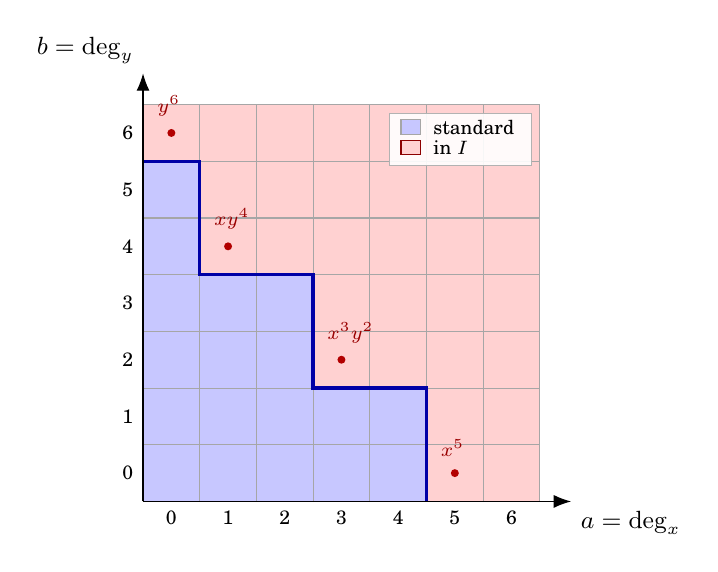
\begin{tikzpicture}[scale=.72, every node/.style={font=\small}]
  
  % In the displayed window, color everything red first: ideal monomials.
  \foreach \a in {0,...,6}{
    \foreach \b in {0,...,6}{
      \fill[red!18] (\a,\b) rectangle +(1,1);
    }
  }

  % Standard monomials: monomials not in I.
  \foreach \b in {0,...,5}{\fill[blue!22] (0,\b) rectangle +(1,1);}
  \foreach \a in {1,2}{
    \foreach \b in {0,...,3}{\fill[blue!22] (\a,\b) rectangle +(1,1);}
  }
  \foreach \a in {3,4}{
    \foreach \b in {0,1}{\fill[blue!22] (\a,\b) rectangle +(1,1);}
  }

  % Grid, axes, and staircase boundary.
  \draw[step=1, black!35, thin] (0,0) grid (7,7);
  \draw[very thick, blue!65!black]
    (0,6) -- (1,6) -- (1,4) -- (3,4) -- (3,2) -- (5,2) -- (5,0);

  \draw[-{Latex[length=2.2mm]}] (0,0) -- (7.55,0) node[below right] {$a=\deg_x$};
  \draw[-{Latex[length=2.2mm]}] (0,0) -- (0,7.55) node[above left] {$b=\deg_y$};

  \foreach \a in {0,...,6}{\node[below] at (\a+.5,0) {\scriptsize \a};}
  \foreach \b in {0,...,6}{\node[left] at (0,\b+.5) {\scriptsize \b};}

  % Minimal generators.
  \foreach \a/\b/\lab in {
    5/0/{$x^5$},
    3/2/{$x^3y^2$},
    1/4/{$xy^4$},
    0/6/{$y^6$}
  }{
    \fill[red!70!black] (\a+.5,\b+.5) circle (2pt);
    \node[anchor=south west, font=\scriptsize, text=red!60!black]
      at (\a+.08,\b+.62) {\lab};
  }

  % Legend.
  \fill[white, fill opacity=.90, draw=black!30] (4.35,5.92) rectangle (6.85,6.85);
  \fill[blue!22, draw=black!35] (4.55,6.48) rectangle +(0.35,0.25);
  \node[anchor=west, font=\scriptsize] at (4.95,6.60) {standard};
  \fill[red!18, draw=red!55!black] (4.55,6.12) rectangle +(0.35,0.25);
  \node[anchor=west, font=\scriptsize] at (4.95,6.24) {in $I$};
\end{tikzpicture}
\end{center}

\begin{definition}
Let $I\subset S$ be an ideal. A monomial $x^{\alpha}$ is called a \emph{standard monomial} for $I$ with respect to $<$ if $x^{\alpha}\notin \init_<(I)$.
\end{definition}

We denote the set of standard monomials by $\std_<(I)$. If $G=\{g_1,\ldots,g_t\}$ is a finite set of nonzero polynomials, we say $x^{\alpha}$ is \emph{standard for $G$} if no $\LM(g_i)$ divides $x^{\alpha}$. If $G$ is a Gr\"obner basis for $I$, then being standard for $I$ is the same as being standard for $G$. Thus the standard monomials can be read off from the leading monomials of any Gr\"obner basis.

\begin{theorem}[Standard Monomial Basis Theorem]\label{thm:standard-basis}
Let $I\subset S$ be an ideal and fix a monomial order. The residue classes of the standard monomials form a $\KK$-basis of $S/I$.
\end{theorem}

\hrulefill

\begin{enumerate}[leftmargin=*, resume=problems]

\item \textbf{Proving the Standard Monomial Basis Theorem.} Let $G=\{g_1,\ldots,g_t\}$ be a Gr\"obner basis for $I$.
\begin{enumerate}[label=(\alph*),ref=\theenumi\alph*]
    \item Show that the remainder obtained by dividing any $f\in S$ by $G$ is a $\KK$-linear combination of standard monomials.
    
    \item Deduce that the residue classes of the standard monomials span $S/I$.
    
    \item Suppose $h$ is a nonzero $\KK$-linear combination of standard monomials. Prove that $h\notin I$. Hint: What can you say about $\LT(h)$ if $h\in I$?
    
    \item Deduce linear independence and conclude Theorem~\ref{thm:standard-basis}.
    
    \item Explain why Theorem~\ref{thm:standard-basis} gives another proof that normal forms with respect to a Gr\"obner basis are unique.
\end{enumerate}

\item \textbf{Computing standard monomials.} In each part, list the standard monomials and draw the staircase picture when there are only two variables.
\begin{enumerate}[label=(\alph*),ref=\theenumi\alph*]
    \item $M=\langle x^3,x^2y,y^4\rangle\subset\KK[x,y]$.
    
    \item $M=\langle x^2,xy,y^3\rangle\subset\KK[x,y]$.
    
    \item $M=\langle x^2z,xyz,y^2z,z^3\rangle\subset\KK[x,y,z]$.
    
    \item Let $I=\langle x-y^2,y^3-1\rangle\subset\KK[x,y]$ with lex order $x>y$. Verify that the displayed generators are a reduced Gr\"obner basis. List $\std_<(I)$ and compute $\dim_{\KK}(S/I)$.
    
    \item With $I$ as in part (d), compute the normal forms of $x^5$, $x^2y+y^7$, and $xy^2+x+y$.
\end{enumerate}

\item \textbf{Finite quotients and powers of variables.} Let $I\subset S$ be an ideal and fix a monomial order.
\begin{enumerate}[label=(\alph*),ref=\theenumi\alph*]
    \item Prove that $S/I$ is finite-dimensional as a $\KK$-vector space if and only if $\std_<(I)$ is finite. In this case,
    \[
    \dim_{\KK}(S/I)=\#\std_<(I).
    \]
    
    \item Let $M\subset S$ be a monomial ideal. Prove that $S/M$ is finite-dimensional over $\KK$ if and only if, for every variable $x_i$, there exists an integer $a_i\geq1$ such that $x_i^{a_i}\in M$.
    
    \item Deduce that $S/I$ is finite-dimensional over $\KK$ if and only if, for every variable $x_i$, there exists $a_i\geq1$ such that $x_i^{a_i}\in \init_<(I)$.
    
    \item Apply part (c) to the ideals
    \[
    \langle x-y^2,y^3-1\rangle,\qquad \langle xy-1\rangle,\qquad \langle x^2,y^2,z^2,xy-yz\rangle.
    \]
\end{enumerate}
\end{enumerate}

\hrulefill

We now turn to the computational heart of the subject. The obstruction to a generating set being a Gr\"obner basis is cancellation of leading terms. Buchberger's insight was that it is enough to check the simplest possible cancellations, namely pairwise cancellations.

\begin{definition}
Let $f,g\in S$ be nonzero. Write $\LT(f)=c_fx^{\alpha}$ and $\LT(g)=c_gx^{\beta}$, and let $x^{\gamma}=\operatorname{lcm}(x^{\alpha},x^{\beta})$. The \emph{$S$-polynomial} of $f$ and $g$ is
\[
    S(f,g)=\frac{x^{\gamma-\alpha}}{c_f}f-\frac{x^{\gamma-\beta}}{c_g}g.
\]
Thus the leading terms of the two summands cancel.
\end{definition}

\begin{theorem}[Buchberger's Criterion]\label{thm:buchberger}
Let $G=\{g_1,\ldots,g_t\}\subset S$ and set $I=\langle G\rangle$. Then $G$ is a Gr\"obner basis for $I$ if and only if every $S(g_i,g_j)$ has remainder zero on division by $G$.
\end{theorem}

\hrulefill

\begin{enumerate}[leftmargin=*, resume=problems]

\item \textbf{$S$-polynomials by hand.} Work in $\KK[x,y]$ with lex order $x>y$.
\begin{enumerate}[label=(\alph*),ref=\theenumi\alph*]
    \item Let $g_1=xy-1$ and $g_2=y^2-1$. Compute $S(g_1,g_2)$ and reduce it by the ordered list $(g_1,g_2)$.
    
    \item Add the nonzero remainder from part (a) to the list. Call it $g_3$. Compute $S(g_1,g_3)$ and $S(g_2,g_3)$ and reduce both by $(g_1,g_2,g_3)$.
    
    \item Conclude that $\{g_1,g_2,g_3\}$ is a Gr\"obner basis for $\langle xy-1,y^2-1\rangle$.
    
    \item Reduce this Gr\"obner basis to the unique reduced Gr\"obner basis.
\end{enumerate}

\item \textbf{Another full Buchberger computation.} Work in $\KK[x,y]$ with lex order $x>y$. Let
\[
    f_1=x^2-y,\qquad f_2=xy-1,
\]
and set $I=\langle f_1,f_2\rangle$.
\begin{enumerate}[label=(\alph*),ref=\theenumi\alph*]
    \item Compute $S(f_1,f_2)$ and reduce it by $(f_1,f_2)$.
    
    \item Continue Buchberger's algorithm until every pair reduces to zero.
    
    \item Show that the reduced Gr\"obner basis is $ \{x-y^2,\; y^3-1\}$.

    \item Find the standard monomials of $S/I$ and to solve the system $x^2-y=xy-1=0$ over $\CC$.
\end{enumerate}

\item \textbf{Proving Buchberger's Criterion.} We prove Theorem~\ref{thm:buchberger} in pieces. Let $G=\{g_1,\ldots,g_t\}$ and $I=\langle G\rangle$.
\begin{enumerate}[label=(\alph*),ref=\theenumi\alph*]
    \item Prove the easy direction: if $G$ is a Gr\"obner basis, then every $S(g_i,g_j)$ reduces to zero modulo $G$.
    
    \item For the converse, let $f\in I$ and write $f=q_1g_1+\cdots+q_tg_t$. For such a representation, define
    \[
    \delta(q_1,\ldots,q_t)=\max_i\LM(q_ig_i).
    \]
    Choose a representation of $f$ for which $\delta$ is as small as possible. Explain why this makes sense.
    
    \item Show that if the terms of monomial $\delta$ in the sum $\sum q_ig_i$ do not cancel, then $\LT(f)$ is divisible by some $\LT(g_i)$.
    
    \item Suppose instead that the terms of monomial $\delta$ cancel. Show that the cancellation gives a nontrivial relation among leading terms of some $g_i$'s.
    
    \item Use the assumption that every $S(g_i,g_j)$ reduces to zero to replace this relation by a combination of the $g_i$'s whose terms all have monomial strictly smaller than $\delta$.
    
    \item Explain why part (e) contradicts the minimal choice of the representation unless $\LT(f)$ is divisible by some $\LT(g_i)$.
    
    \item Conclude that $\init_<(I)=\langle \LT(g_1),\ldots,\LT(g_t)\rangle$.
\end{enumerate}

\item \textbf{Buchberger's Algorithm.} Buchberger's criterion leads directly to an algorithm.
\begin{algorithm}[H]
\caption{Buchberger's Algorithm}
\begin{algorithmic}[1]
\State \textbf{Input:} nonzero polynomials $F=\{f_1,\ldots,f_s\}\subset S$ and a monomial order $<$
\State $G\gets F$
\State $P\gets \{\{g,h\}\mid g,h\in G,\; g\neq h\}$
\While{$P\neq\varnothing$}
    \State choose a pair $\{g,h\}\in P$ and remove it from $P$
    \State divide $S(g,h)$ by $G$ and let $r$ be the remainder
    \If{$r\neq0$}
        \State $P\gets P\cup \{\{r,k\}\mid k\in G\}$
        \State $G\gets G\cup\{r\}$
    \EndIf
\EndWhile
\State \textbf{return} $G$
\end{algorithmic}
\end{algorithm}

\begin{enumerate}[label=(\alph*),ref=\theenumi\alph*]
    \item Prove that whenever a nonzero remainder $r$ is added, the monomial ideal $\langle \LT(g)\mid g\in G\rangle$ strictly increases.
    
    \item Use the Noetherian property of $S$ (or Dickson's Lemma for monomial ideals) to prove that the algorithm terminates.
    
    \item Prove that the output is a Gr\"obner basis for $\langle F\rangle$.
\end{enumerate}


\item \textbf{Ideal membership, inclusion, and equality.} Let $I=\langle f_1,\ldots,f_s\rangle$ and $J=\langle h_1,\ldots,h_r\rangle$ be ideals of $S$.
\begin{enumerate}[label=(\alph*),ref=\theenumi\alph*]
    \item Suppose $G_J$ is a Gr\"obner basis for $J$. Prove that $I\subseteq J$ if and only if every $\NF_{G_J}(f_i)=0$.
    
    \item Explain how to test whether $I=J$ using two Gr\"obner basis computations.
    
    \item Use part (a) to decide whether
    \[
    \langle x^2-y,xy-1\rangle \subseteq \langle x-y^2,y^3-1\rangle
    \]
    in $\KK[x,y]$ with lex order $x>y$.
    
    \item Let $G$ be a Gr\"obner basis for $I$. Prove that $f$ and $g$ have the same image in $S/I$ if and only if $\NF_G(f)=\NF_G(g)$.
\end{enumerate}

\item \textbf{Radical membership: the Rabinowitsch trick.} Let $I=\langle f_1,\ldots,f_s\rangle\subset S$ and let $f\in S$. Introduce a new variable $u$.
\begin{enumerate}[label=(\alph*),ref=\theenumi\alph*]
    \item Prove that
    \[
    f\in \sqrt{I}
    \quad\Longleftrightarrow\quad
    1\in \langle f_1,\ldots,f_s,1-uf\rangle\subset S[u].
    \]
    Hint: Interpret $S[u]/\langle 1-uf\rangle$ as the localization $S[f^{-1}]$.
    
    \item Explain how this turns radical membership into an ideal membership test using a Gr\"obner basis.
    
    \item Use this criterion to show that $x\in \sqrt{\langle x^2,xy\rangle}\subset \KK[x,y]$.
    
    \item Is $y\in \sqrt{\langle x^2,xy\rangle}$? Justify your answer algebraically and with the Gr\"obner basis criterion.
\end{enumerate}

\item \textbf{Computer check.} Use \textit{Macaulay2} to verify at least two computations from this worksheet.
\begin{enumerate}[label=(\alph*),ref=\theenumi\alph*]
    \item Compute a Gr\"obner basis for $\langle xy-1,y^2-1\rangle$ with lex order $x>y$.
    
    \item Compute a Gr\"obner basis for $\langle x^2-y,xy-1\rangle$ with lex order $x>y$.
    
    \item Compute the standard monomials for one zero-dimensional ideal above.
    
    \item Compute one intersection ideal from Problems 15 and 16.
    
    \item Compare the reduced Gr\"obner basis returned by the computer with your hand computation. Which intermediate choices differed, and why did the reduced answer not depend on those choices?
\end{enumerate}

\end{enumerate}


\end{document}
